\section{The \SYSTEM{} Approach} \label{sec:approach}

In this section we detail the \SYSTEM{} approach, a practical defense against
receiving corrupted or compromised resources over the internet that 1) is
automated to account for user apathy and 2) does not require co-hosting the
checksum, which creates a single point of failure and renders checksum
verification (even automated checksum verification) irrelevant.

The \SYSTEM{} approach is not limited to browsers. It can also be incorporated
into, for instance, FTP and SSH clients (\eg{rsync}), mobile apps, etc.

\TODO{General high level description of function.} 1) the unique identification
of individual hosted resources and 2) a high availability mapping of unique
resource identifiers to corresponding checksums.

\SYSTEM{} implementations can be imagined as a security layer sitting between
the user and the resource. Immediately after a resource is downloaded, two
cryptographic digests are generated. One digest uniquely fingerprints said
resource based on its name. This is known as the \emph{Non-Authoritative
Checksum} (NAC) and is yielded from running the cryptographic hashing function
over the contents of the resource file. The second digest uniquely fingerprints
said resource based on its contents. This is known as the \emph{Resource
Identifier} (RI) and is yielded from running the cryptographic hashing function
over the resource's public path on the distribution system.

Next, \SYSTEM{} uses the RI to retrieve an \emph{Authoritative Checksum} (AC)
from the backend. If successful, \SYSTEM{} will compare the NAC to the AC---we
refer to this as \emph{Non-Authoritative Checksum Validation} (NAC Validation).
In the case where NAC Validation fails, \ie they do not match, some
implementation-specific action should be taken to mitigate as much as possible
the risk to the end user. In most contexts, this means deleting or renaming the
unsafe resource, forcing the user to deal with the problem. Otherwise, \SYSTEM{}
remains completely transparent the the end user, as demonstrated by our
browser-based implementations.

\TODO{Re-explain/highlight why web server compromise alone doesn’t defeat HASCHK}

\subsection{Accounting for User Apathy}

Human factors such as user apathy have stymied cryptographers for decades.
Schemes that are otherwise reasonably cryptographically solid can fail
catastrophically due to human error, confusion, aversion to inconvenience, or
simple lack of interest. Some users are likely to avoid using a security measure
altogether if it presents even a minor obstacle to immediate
gratification~\cite{Clickthrough, PGPBad, Egelman1, Egelman2, Jenkins, Modic,
Reeder, Silic, Sunshine, Bianchi, Akhawe, Cherubini}.

\PUNT{\begin{figure}[t]
    \centering
    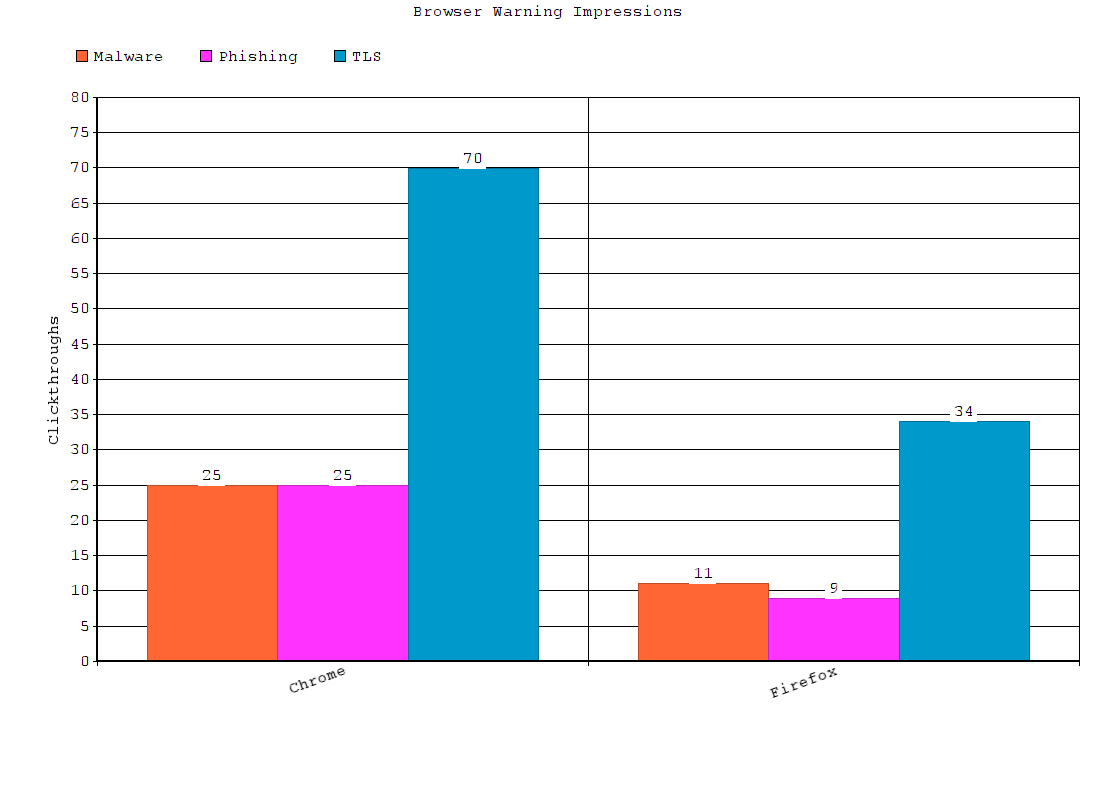
\includegraphics[width=0.95\linewidth]{impressions.png}
    \caption{Akhawe et al. estimation of warning clickthroughs by users as a
    percentage of total warnings observed for two popular
    browsers.}\label{fig:telemetry}
\end{figure}}

With this in mind, the primary goal of \SYSTEM{} is to side-step the human
factor altogether by providing a completely transparent and unobtrusive,
fully-automated method of checksum calculation and verification in the average
case. In a non-average case (\ie{when a download fails its integrity check}), we
1) clearly, visibly, and simply assert the danger of the download and 2)
privilege security over choice by rejecting the download by default and making
it inconvenient to ignore or click through the resulting security warning. In
this way, the security measure cannot be avoided.

Our \DNSSYS{} and \DHTSYS{} implementations were designed with this guidance in
mind, with ideal implementations able to rely on Google Chrome's dangerous
download UI~\cite{ChromeClickThrough}. \TODO{talk about how the dangerous
download UI is "from an authority," is harder to click through, and that this is
verified by the Chrome dev team}.

\subsection{Mitigating the Co-Hosting Problem}

Funding and maintaining a single server/system to host assets can be extremely
cost-effective in the short term compared to hosting two or more discrete
systems, such as one to host a resource and another to host a resource's
checksum. Unfortunately, this creates a single point of failure: an attacker
that compromises this system can both corrupt the resource and update the
checksum to match. Hence, \emph{co-hosting} a resource and its
corresponding checksum on the same distribution system virtually negates the
effectiveness of having a checksum at all. This is widely understood in the
security community~\cite{SCA-MINT2, Cherubini, Stickler}.

Hence, deployment of \SYSTEM{} necessitates the existence of a separate
distribution mechanism for resources and for authoritative checksums. The idea
of using some distributed storage service to query a global mapping between
between resource and checksum is not new and may seem straightforward, but the
problem is deceptively complex.

Fortunately, there has been a lot of effort put into researching, designing, and
standardizing several high availability high performance storage technologies,
some of which web-facing entities and IT teams are already quite familiar with
and most already pay for, \eg the Domain Name System (DNS). Adding extra
resource records to a DNS zone, for instance, is essentially a costless
operation, meaning any entity that already has a web presence can immediately
deploy \SYSTEM{}'s \DNSSYS{} implementation. This is key to the motivation
behind the \SYSTEM{} approach and the design of \DNSSYS{}.

Other candidate high availability systems include DHTs, storage clusters,
relational and non-relational databases, and any high availability key-value
store.

\TODO{Note we beat Stickler and Cherubini et al because we can survive server compromise}
